%%%%%%%%%%%%%%%%%%%%%%%%%%%%%%%%%%%%%%%%
%%%%%  Chapitre Liens 
%%%%%%%%%%%%%%%%%%%%%%%%%%%%%%%%%%%%%%%%

\chapter{Liens avec d'autres programmes}

\section{Conversion d'image} \index[con]{image} \label{conversionimage}

Dans le cadre de la chaîne de compilation \programme{ps2pdf} vue en page \pageref{compilations}, \LaTeX\ n'accepte que des images au format \dextension{eps}. Pour convertir un fichier image en fichier \dextension{eps}, de nombreux programmes sont disponibles. En voici un exemple avec le logiciel libre \programme{The Gimp}\footnote{Il est téléchargeable à l'adresse \liensimple{http://www.gimp.org/}.}.

Après avoir ouvert une image éditable avec \programme{The Gimp}, il faut aller dans le menu \vue{Fichier}, \vue{Exporter...} et le formulaire suivant apparaît. 

\begin{figure}[H]
\centering
\resizebox{9cm}{!}{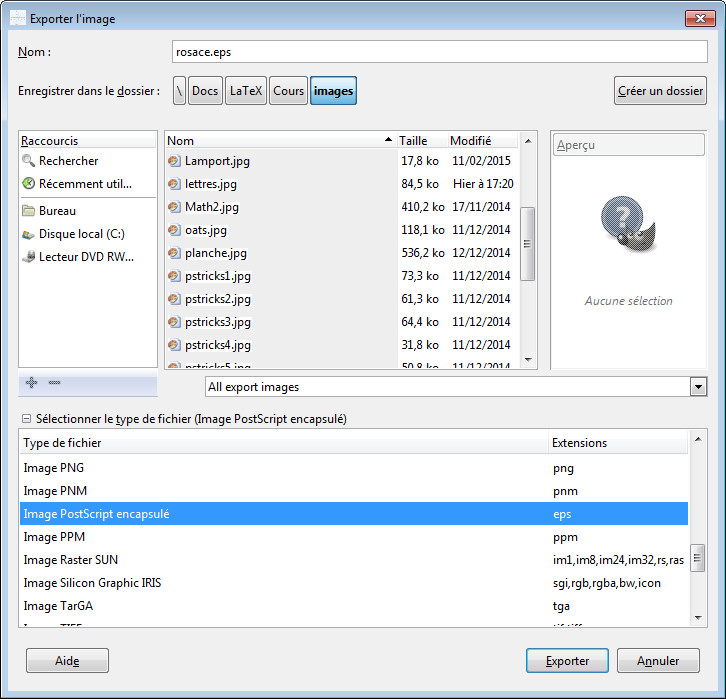
\includegraphics{images/thegimp1.jpg}}
\caption{Formulaire d'exportation de \programme{The Gimp}}
\end{figure}

Il suffit alors de changer le type de l'image en cliquant sur \vue{Sélectionner le type de fichier} puis \vue{Image postscript encapsulé} et enfin \vue{Exporter}. Dans la plupart des cas, les options proposées par défaut dans le second formulaire qui apparaît ne sont pas à modifier.

\begin{figure}[H]
\centering
\resizebox{8cm}{!}{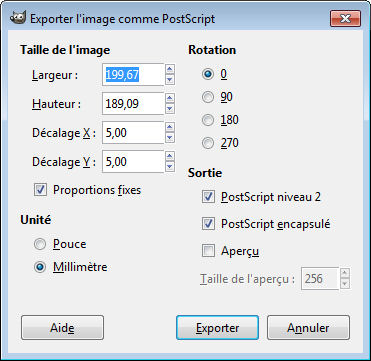
\includegraphics{images/thegimp2.jpg}}
\caption{Formulaire des options \dextension{eps} de \programme{The Gimp}}
\end{figure}

La figure s'insère alors dans \LaTeX\ en suivant la logique présentée en section \ref{images}.

\section{\programme{Excel}}

Comme vu en \ref{macroexcel} page \pageref{macroexcel}, la macro complémentaire \programme{Excel2LaTeX} permet de convertir une zone d'une feuille \programme{Excel} en un code \LaTeX\ générant un tableau simple.

Mais la transmission d'information entre \programme{Excel} et \LaTeX\ peut aller plus loin. \LaTeX\ travaille en effet sur des fichiers en format texte, format générable et manipulable par la plupart des langages de programmation, tel le \programme{Visual Basic}. Voici donc un exemple de code \programme{Visual Basic} permettant ceci :

\begin{codesimple}{Macro VB créant un code \LaTeX\ en encodage latin1}{macrovb}
Sub Test()
Open "C:\Test\liste.tex" For Output As #1
Avertissement = Cells(1, 1)
Signature = Cells(2, 1)
Print #1, "Attention :"
Print #1, "\begin{center}"
Print #1, Avertissement
Print #1, "\textsc{" & Signature & "}"
Print #1, "\end{center}"
Close #1
End Sub
\end{codesimple}

La procédure \macron{Test}, avec la commande \macron{Open For Output As \#1}, va accéder en mémoire au fichier \vue{liste.tex} dans le répertoire indiqué. Si le fichier n'existe pas, Excel le crée\footnote{Mais si le répertoire n'existe pas, \programme{Excel} ne le crée ici pas.}. Ce code récupère avec les deux lignes suivantes les valeurs présentes dans deux cellules de la feuille \programme{Excel} active. Chaque ligne commençant par \macron{Print \#1,} insère alors la suite de la ligne dans le fichier \vue{liste.tex}. La commande \vue{Close \#1} referme enfin le fichier \vue{liste.tex}.

Les différentes lignes commençant par \macron{Print \#1,} insèrent des chaînes de caractère encadrées par le caractère \macron{"} ou des variables. La concaténation de chaînes de caractère ou de variables se fait avec le caractère \macron{\&}\footnote{Ceci est vrai dans le code \programme{Visual Basic} tout comme dans les formules apparaissant dans une feuille \programme{Excel}.}.

Le fichier \vue{liste.tex} peut alors être compilé avec \LaTeX\ s'il est complet ou être intégré dans un autre fichier avec les commandes \macro{include} ou \macro{input}, comme indiqué en section \ref{scission}, page \pageref{scission}.

Pour travailler en UTF8, le code à retenir est plus complexe (mais aussi plus général) :

\begin{codesimple}{Macro VB créant un code \LaTeX\ en encodage UFT8}{macrovbutf8}
Sub Test()
' On teste l'existence du fichier final (pour le supprimer)
Set objFSO = CreateObject("Scripting.FileSystemObject")
If objFSO.FileExists("C:\Test\liste.tex") Then Kill ("C:\Test\liste.tex")
    
' Creation de l'objet contenant le texte LaTeX
Dim objStream As Object                       ' Définition
Set objStream = CreateObject("ADODB.Stream")  ' Création
objStream.Open                                ' Ouverture
objStream.Position = 0                        ' On se place au début
objStream.Charset = "UTF-8"                   ' Encodage UTF8
    
Avertissement = Cells(1, 1)
Signature = Cells(2, 1)    
objStream.WriteText "Attention :" & vbCr
objStream.WriteText "\begin{center}" & vbCr
objStream.WriteText Avertissement & vbCr
objStream.WriteText "\textsc{" & Signature & "}" & vbCr
objStream.WriteText "\end{center}" & vbCr

' Sauvegarde finale et fermeture de l'objet créé
objStream.SaveToFile "C:\Test\liste.tex"
objStream.Close
End Sub
\end{codesimple}

Ici, le \macron{vbCr} permet d'insérer un retour à la ligne.

\section{Les logiciels mathématiques}

La précision de \LaTeX\ en matière de mathématiques en a fait un des outils les plus appréciés des mathématiciens. Aussi, de nombreuses applications mathématiques proposent la génération de codes ou de figures réutilisables immédiatement par \LaTeX.


\subsection{\programme{R}, avec \programme{Sweave}}

L'extension \programme{Sweave} du logiciel \programme{R} permet de créer un document \dextension{tex} sur la base d'un document d'extension dédiée \dextension{Snw} (ou \dextension{Rnw}) placé dans le répertoire de travail usuel de \programme{R}. Ce document contient du code \LaTeX\ classique mais peut contenir aussi du code \programme{R} en respectant la norme suivante :

\begin{codesimple}{Encadrement d'un code \programme{R} sous \LaTeX}{encadrer}
<<§oc paramètres d'affichage §fc >>= 
§oc Lignes de code R §fc
@
\end{codesimple}


En voici quelques exemples appliqués :

\begin{codesimple}{Exemples de code \programme{R} sous \LaTeX}{exempler}
<<>>=  
library(stats)
x <- rnorm(20)
print(x)
print(t1 <- t.test(x))
@ 

<<echo=TRUE,print=TRUE>>= 
1 + 1          
1 + pi        
sin(pi/2) 
@
\end{codesimple}


Sous \programme{R}, ce document est exécutable avec \programme{Sweave} en utilisant la série de commandes suivantes :

\begin{codesimple}{Instructions sous \programme{R}}{instructionsr}
test <- system.file("Sweave", "§oc fichier§fc£¤.Snw", package = "utils")  \\
Sweave(test)
\end{codesimple}


Une fois que \programme{R} a effectué son traitement, il restitue un fichier \dextension{tex} et autant d'images \dextension{pdf} ou d'images \dextension{eps}\footnote{Pour obtenir des images \dextension{eps}, le fichier \dextension{Snw} doit contenir l'instruction \macro{SweaveOpts\{eps=true\}}.} que de figures demandées à \programme{R}. Le document \LaTeX\ doit contenir dans son préambule l'appel suivant :

\begin{codesimple}{Paquet nécessaire pour travailler avec \programme{R} et \programme{Sweave}}{sweave}
\usepackage{Sweave}
\end{codesimple}


Le paquet \paquet{Sweave} se trouve dans les répertoires de \programme{R} et peut être copié dans le même répertoire que votre fichier \dextension{tex}. La suite revient à l'utilisation classique de \LaTeX.

Les possibilités sont ici nombreuses et, pour une vision bien plus complète, il existe un document de Jean Raymond \textsc{Lobry}\cite{lobr} sur la question.
